\documentclass{beamer}

\usefonttheme{serif}
\usepackage{dsfont}
\setbeamersize{text margin left=5pt, text margin right=5pt}

\newcommand{\bgk}[1]{\boldsymbol{#1}}

\newcommand{\bzero}{\bgk{0}}
\newcommand{\bone}{\bgk{1}}

\newcommand{\balpha}{\bgk{\alpha}}
\newcommand{\bnu}{\bgk{\nu}}
\newcommand{\bbeta}{\bgk{\beta}}
\newcommand{\bxi}{\bgk{\xi}}
\newcommand{\bgamma}{\bgk{\gamma}} 
\newcommand{\bo}{\bgk{o }}
\newcommand{\bdelta}{\bgk{\delta}}
\newcommand{\bpi}{\bgk{\pi}}
\newcommand{\bepsilon}{\bgk{\epsilon}} 
\newcommand{\bvarepsilon}{\bgk{\varepsilon}} 
\newcommand{\brho}{\bgk{\rho}}
\newcommand{\bvarrho}{\bgk{\varrho}}
\newcommand{\bzeta}{\bgk{\zeta}}
\newcommand{\bsigma}{\bgk{\sigma}}
\newcommand{\boldeta}{\bgk{\eta}}
\newcommand{\btay}{\bgk{\tau}}
\newcommand{\btheta}{\bgk{\theta}}
\newcommand{\bvertheta}{\bgk{\vartheta}}
\newcommand{\bupsilon}{\bgk{\upsilon}}
\newcommand{\biota}{\bgk{\iota}}
\newcommand{\bphi}{\bgk{\phi}}
\newcommand{\bvarphi}{\bgk{\varphi}}
\newcommand{\bkappa}{\bgk{\kappa}}
\newcommand{\bchi}{\bgk{\chi}}
\newcommand{\blambda}{\bgk{\lambda}}
\newcommand{\bpsi}{\bgk{\psi}}
\newcommand{\bmu}{\bgk{\mu}}
\newcommand{\bomega}{\bgk{\omega}}

\newcommand{\bA}{\bgk{A}}
\newcommand{\bDelta}{\bgk{\Delta}}
\newcommand{\bLambda}{\bgk{\Lambda}}
\newcommand{\bSigma}{\bgk{\Sigma}}
\newcommand{\bOmega}{\bgk{\Omega}}

\newcommand{\bvec}[1]{\mathbf{#1}}

\newcommand{\va}{\bvec{a}}
\newcommand{\vb}{\bvec{b}}
\newcommand{\vc}{\bvec{c}}
\newcommand{\vd}{\bvec{d}}
\newcommand{\ve}{\bvec{e}}
\newcommand{\vf}{\bvec{f}}
\newcommand{\vg}{\bvec{g}}
\newcommand{\vh}{\bvec{h}}
\newcommand{\vi}{\bvec{i}}
\newcommand{\vj}{\bvec{j}}
\newcommand{\vk}{\bvec{k}}
\newcommand{\vl}{\bvec{l}}
\newcommand{\vm}{\bvec{m}}
\newcommand{\vn}{\bvec{n}}
\newcommand{\vo}{\bvec{o}}
\newcommand{\vp}{\bvec{p}}
\newcommand{\vq}{\bvec{q}}
\newcommand{\vr}{\bvec{r}}
\newcommand{\vs}{\bvec{s}}
\newcommand{\vt}{\bvec{t}}
\newcommand{\vu}{\bvec{u}}
\newcommand{\vv}{\bvec{v}}
\newcommand{\vw}{\bvec{w}}
\newcommand{\vx}{\bvec{x}}
\newcommand{\vy}{\bvec{y}}
\newcommand{\vz}{\bvec{z}}

\newcommand{\vA}{\bvec{A}}
\newcommand{\vB}{\bvec{B}}
\newcommand{\vC}{\bvec{C}}
\newcommand{\vD}{\bvec{D}}
\newcommand{\vE}{\bvec{E}}
\newcommand{\vF}{\bvec{F}}
\newcommand{\vG}{\bvec{G}}
\newcommand{\vH}{\bvec{H}}
\newcommand{\vI}{\bvec{I}}
\newcommand{\vJ}{\bvec{J}}
\newcommand{\vK}{\bvec{K}}
\newcommand{\vL}{\bvec{L}}
\newcommand{\vM}{\bvec{M}}
\newcommand{\vN}{\bvec{N}}
\newcommand{\vO}{\bvec{O}}
\newcommand{\vP}{\bvec{P}}
\newcommand{\vQ}{\bvec{Q}}
\newcommand{\vR}{\bvec{R}}
\newcommand{\vS}{\bvec{S}}
\newcommand{\vT}{\bvec{T}}
\newcommand{\vU}{\bvec{U}}
\newcommand{\vV}{\bvec{V}}
\newcommand{\vW}{\bvec{W}}
\newcommand{\vX}{\bvec{X}}
\newcommand{\vY}{\bvec{Y}}
\newcommand{\vZ}{\bvec{Z}}

\usepackage{subcaption}
\newcommand{\bitem}{\item[$\bullet$]}

\usepackage{xcolor}
\usepackage[utf8]{inputenc}
\DeclareFontEncoding{LS1}{}{}
\DeclareFontSubstitution{LS1}{stix}{m}{n}
\DeclareSymbolFont{symbols2}{LS1}{stixfrak} {m} {n}
\DeclareMathSymbol{\operp}{\mathbin}{symbols2}{"A8}
\setbeamertemplate{navigation symbols}{}

\usepackage{lipsum}

\newcommand\blfootnote[1]{%
  \begingroup
  \renewcommand\thefootnote{}\footnote{#1}%
  \addtocounter{footnote}{-1}%
  \endgroup
}

\addtobeamertemplate{navigation symbols}{}{%
    \usebeamerfont{footline}%
    \usebeamercolor[fg]{footline}%
    \hspace{1em}%
    \insertframenumber/\inserttotalframenumber
}

\title{
Monte Carlo Integration\\
Lecture 3
}
%\subtitle{Mathematical framework, existence and exactness}

\author{F. M. Faulstich}
\date{01/16/2024}


\begin{document}

\frame{\titlepage}

\begin{frame}{Numerical intergration}

Why do we care?\\
~\\
\pause
\only<2>{
Application in Quantum Chemistry:
$$
v_{p,q,r,s}
=
\int_{\mathbb{R}^3}
\int_{\mathbb{R}^3}
\frac{\chi_p(\vr_1)\chi_r(\vr_1)\chi_q(\vr_2)\chi_s(\vr_2)}{|\vr_1 - \vr_2|} d\vr_1 d\vr_2
$$
}
\only<3>{
Discretization of continuous operators:
$$
[\vD]_{i,j} = \int_{X} \phi_i(\vx)\, \mathcal{D}\, \phi_j(\vx) d\vx 
$$
}
\only<4>{
Numerically solving differential equations:
\begin{itemize}
    \bitem Left Riemann sum $\rightarrow$ explicit Euler 
    \bitem Right Riemann sum $\rightarrow$ implicit Euler
    \bitem Trapezoidal rule $\rightarrow$ Crank-Nicolson
    \item[~] $\vdots$
\end{itemize}
}

\end{frame}

\begin{frame}{Numerical integration}
We are interested in computing
$$
F=\int_a^b f(x)~dx
$$
\pause
% Standard numerical techniques
\only<2>{
Riemann sum (Left):
\begin{center}
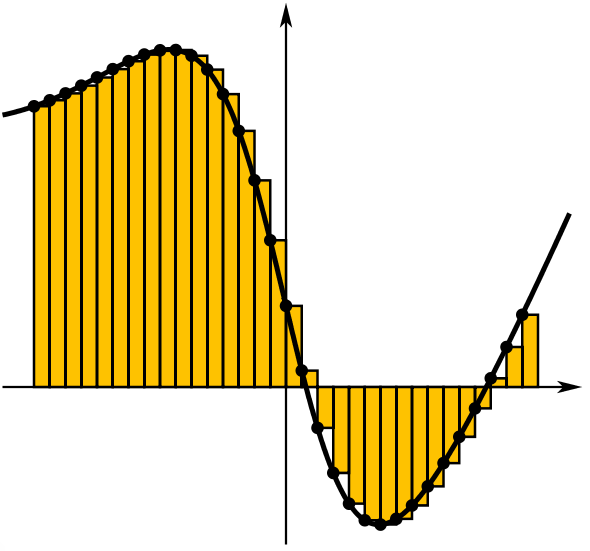
\includegraphics[width = 0.4 \textwidth]{Graphics/RiemanSum1.png}
\end{center}
}

\only<3>{

Let $f:[a,b] \to \mathbb{R}$ be a function defines on a closed interval $[a,b]\subset \mathbb{R}$ and let $\{x_0,...,x_n\}$ be a partition of $[a,b]$, i.e.,
$$
a = x_0 <x_1 <...<x_n = b.
$$
Then
$$
R_{\rm left} (f,n)
=
\sum_{i=1}^{n} f(x_{i-1}) \Delta x_i
$$
where $\Delta x_i = x_i - x_{i-1}$
}

\only<4>{

Riemann sum (Right):
\begin{center}
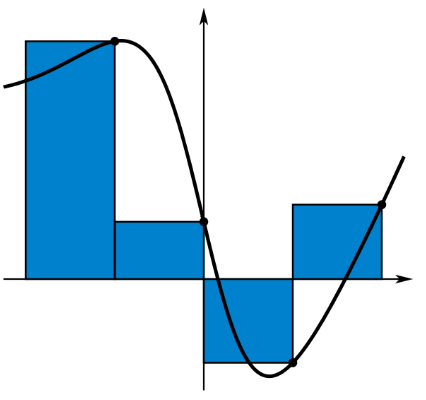
\includegraphics[width = 0.4 \textwidth]{Graphics/RiemanSum2.png}
\end{center}

}

\only<5>{

Riemann sum (Upper):
\begin{center}
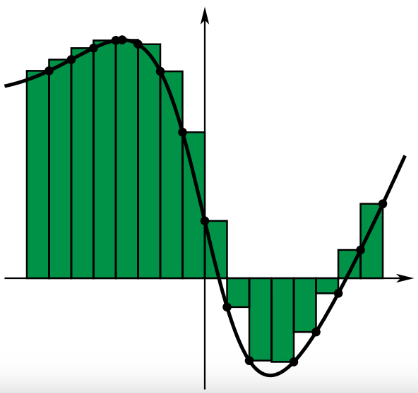
\includegraphics[width = 0.4 \textwidth]{Graphics/RiemanSum3.png}
\end{center}

}

\only<6>{

Riemann sum (Lower):
\begin{center}
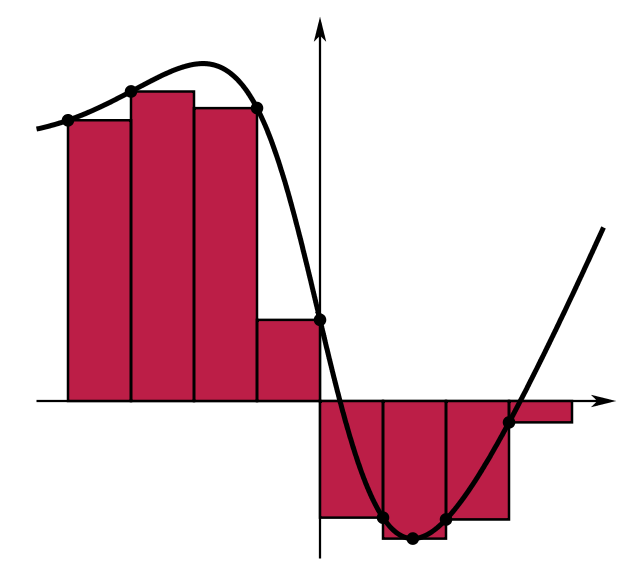
\includegraphics[width = 0.4 \textwidth]{Graphics/RiemanSum4.png}
\end{center}

}


\end{frame}


\begin{frame}{Riemann Sums}

Let $f:[a,b] \to \mathbb{R}$ be a function defines on a closed interval $[a,b]\subset \mathbb{R}$ and let $\{x_0,...,x_n\}$ be a partition of $[a,b]$, i.e.,
$$
a = x_0 <x_1 <...<x_n = b.
$$
Then
$$
R(f,n)
=
\sum_{i=1}^{n} f(\tilde{x}_{i}) \Delta x_i
$$
where $\Delta x_i = x_i - x_{i-1}$ and $\tilde{x}_i \in [x_{i-1}, x_i]$.

\begin{itemize}
    \bitem Left Riemann sum: If $\tilde{x}_i = x_{i-1}$ 
    \bitem Right Riemann sum: If $\tilde{x}_i = x_i$
    \bitem Upper Riemann sum: If $\tilde{x}_i = \sup(f([x_{i-1}, x_i])$ 
    \bitem Lower Riemann sum: If $\tilde{x}_i = \inf(f([x_{i-1}, x_i])$ 
    \bitem Middle Riemann sum: If $\tilde{x}_i = (x_i + x_{i-1})/2$
\end{itemize}
    
\end{frame}

\begin{frame}{Middle Riemann sum error}

\pause

\begin{itemize}
    \bitem Let $f:[a,b] \to \mathbb{R}$ be a twice continuous differentiable function and 
    $$
    M = \sup_{x\in [a,b]} |f''(x)|
    $$
    Then
    $$
    |R_{\rm mid}(f,n) - F| \leq \frac{M (b-a)^3}{24n^2} \sim \mathcal{O}\left( \frac{1}{n^2}\right)
    $$
\end{itemize}

    
\end{frame}


\begin{frame}{Trapezoidal rule}

We are interested in computing
$$
F=\int_a^b f(x)~dx
$$
Trapezoidal rule:\\
~\\
\only<1>{

\begin{center}
    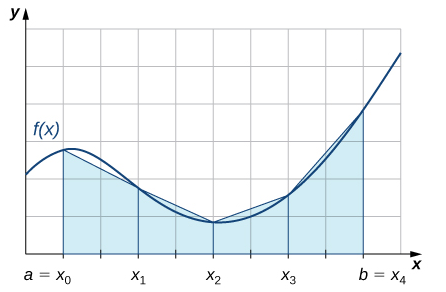
\includegraphics[width = 0.5 \textwidth]{Graphics/TrpezoidalRule.png}
\end{center}

}

\only<2>{

Let $f:[a,b] \to \mathbb{R}$ be a function defines on a closed interval $[a,b]\subset \mathbb{R}$ and let $\{x_0,...,x_n\}$ be a partition of $[a,b]$, i.e.,
$$
a = x_0 <x_1 <...<x_n = b.
$$
Then
$$
T(f,n)
=
\frac{\Delta x}{2}
\left(
f(x_0)+
2\sum_{i=1}^{n-1} f(x_i)
+f(x_n)
\right)
$$

}
    
\end{frame}

\begin{frame}{Trapezoidal rule error}

\begin{itemize}
    \bitem Let $f:[a,b] \to \mathbb{R}$ be a twice continuous differentiable function and 
    $$
    M = \sup_{x\in [a,b]} |f''(x)|
    $$
    Then
    $$
    |T(f,n) - F| \leq \frac{M (b-a)^3}{12 n^2} \sim \mathcal{O}\left( \frac{1}{n^2}\right)
    $$
\end{itemize}
    
\end{frame}

\begin{frame}{Simpson's rule}

We are interested in computing
$$
F=\int_a^b f(x)~dx
$$
~\\
Simpson's rule:
\only<1>{

\begin{center}
    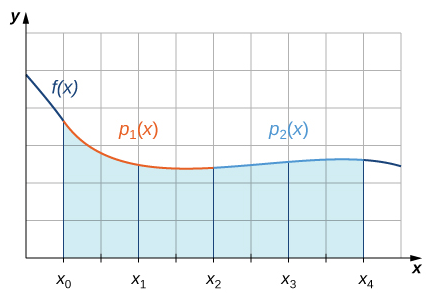
\includegraphics[width = 0.5 \textwidth]{Graphics/Simpson.png}
\end{center}

}

\only<2>{
Let $f:[a,b] \to \mathbb{R}$ be a function defines on a closed interval $[a,b]\subset \mathbb{R}$ and let $\{x_0,...,x_n\}$ be a partition of $[a,b]$ with $n$ even, i.e.,
$$
a = x_0 <x_1 <...<x_n = b.
$$
Then
$$
S(f,n)
=
\frac{\Delta x}{3}
\left(
f(x_0) + 
4 \sum_{i = 0}^{n/2-1} f(x_{2i+1}) + 
2\sum_{i = 1}^{n/2-1} f(x_{2i}) + 
f(x_n)
\right)
$$
}
    
\end{frame}


\begin{frame}{Simpson's rule error}

\begin{itemize}
    \bitem Let $f:[a,b] \to \mathbb{R}$ be a four-times continuously differentiable function and 
    $$
    M = \sup_{x\in [a,b]} |f''(x)|
    $$
    Then
    $$
    |S(f,n) - F| \leq \frac{M (b-a)^5}{180 n^4} \sim \mathcal{O}\left( \frac{1}{n^4}\right)
    $$
\end{itemize}
    
\end{frame}

\begin{frame}{Other classical techniques}
Gaussian quadrature:
$$
F = \sum_{i=1}^n w_i f(x_i)
$$
\begin{itemize}
    \bitem Gauss–Legendre quadrature
    \bitem Gauss–Jacobi quadrature
    \bitem Chebyshev–Gauss quadrature
    \bitem Gauss–Laguerre quadrature
    \bitem Gauss–Hermite quadrature
\end{itemize}

\end{frame}

\begin{frame}{}

\begin{center}
\begin{large}
How does randomness come into play?
\end{large}    
\end{center}

\end{frame}


\begin{frame}{Monte Carlo Estimator}
We are interested in computing
$$
F=\int_a^b f(x)~dx
$$

Idea:\\ 

\only<1>{

\begin{center}
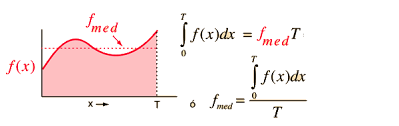
\includegraphics[width = 0.5\textwidth]{Graphics/AverageFunc.png}
\end{center}

}

\only<2>{
We approximate $F$ by averaging samples of the function $f$ at uniform random points in $[a,b]$. \\
~\\
Formally: Given $N$ uniform random variables $X_i \sim \mathcal{U}(a,b)$, its PDF is 
$$
\rho(x)
=
\frac{1}{b-a}\mathds{1}_{[a,b]}(x)
$$
and define the Monte Carlo estimator as
$$
\left\langle
F^N
\right\rangle
=
(b-a) \frac{1}{N} \sum_{i=1}^{N} f(X_i)
$$
}
\end{frame}


\begin{frame}{Expectation value and convergence}
Note:\\
The MC estimator is a random variable itself.\\ 
What is its expectation value?\\
~\\
\pause
Expectation value of the MC estimator
\begin{equation*}
\begin{aligned}
\mathbb{E}(\left\langle
F^N
\right\rangle)
&=
\mathbb{E}
\left(
(b-a) \frac{1}{N} \sum_{i=1}^{N} f(X_i)
\right)
=
(b-a) \frac{1}{N} \sum_{i=1}^{N} 
\mathbb{E}
\left(
f(X_i)
\right)\\
&=
(b-a) \frac{1}{N} \sum_{i=1}^{N} 
\int_{-\infty}^\infty
f(x) \rho(x)~dx=
\frac{1}{N} \sum_{i=1}^{N} 
\int_a^b
f(x)~dx\\
&=
\int_a^b
f(x)~dx = F\\
\end{aligned}
\end{equation*}
What does $N\to \infty$ mean?

\end{frame}



\begin{frame}{Law of large numbers}

Let $X_1,X_2,...$ be an infinite sequence of i.i.d. random variables with 
$$
\mathbb{E}(X_1) = \mathbb{E}(X_2) = ... = \mu
$$
and 
$$
\mathbb{V}(X_1) = \mathbb{V}(X_2) =...= \sigma^2.
$$
Then
\begin{enumerate}
    \item Weak law of large numbers:\\
    For any $\varepsilon >0$
    $$
    \lim_{N \to \infty} \mathbb{P}\left(
    | \bar{X}_N - \mu|< \varepsilon\right)
    = 1
    $$
    (convergence in probability)
    \item Strong law of large numbers:\\
    $$
    \mathbb{P} \left( 
    \lim_{N \to \infty} \bar{X}_N = \mu
    \right) = 1
    $$
    (converges almost surely)
\end{enumerate}

\end{frame}

\begin{frame}{Convergence of Monte-Carlo estimator}
The random variables 
$$
Y_i = (b-a)f(X_i)
$$
are i.i.d. with 
\begin{align*}
\mathbb{E}(Y_i)
&=
\mathbb{E}((b-a)f(X_i))
=
(b-a)\int_{-\infty}^\infty
f(x)\rho(x)dx
=
\frac{b-a}{(b-a)}
\int_a^b
f(x)dx\\
&=
F
\end{align*}
Strong Law of Large Numbers:
$$
\mathbb{P}\left(
\lim_{N\to \infty} 
\left\langle
F^N
\right\rangle = F
\right) 
=
\mathbb{P}\left(
\lim_{N\to \infty} \frac{1}{N}\sum_{i=1}^N Y_i
= F
\right) 
= 1
$$
The MC estimator converges almost surely to the integral $F$.
\end{frame}







\begin{frame}{Rate of convergence}

How quickly does this estimate converge? $\rightarrow$ standard deviation
\begin{equation*}
\begin{aligned}
\mathbb{V}(\left\langle
F^N
\right\rangle)
&=
\mathbb{V}\left(
(b-a) \frac{1}{N} \sum_{i=1}^{N} f(X_i)
\right)
=
\frac{(b-a)^2}{N^2} 
\sum_{i=1}^{N} 
\underbrace{\mathbb{V}\left(
f(X_i)
\right)}_{=: s^2}\\
&=
\frac{(b-a)^2 s^2}{N} 
% &=
% \frac{(b-a)^2}{N^2} 
% \sum_{i=1}^{N} 
% \int_a^b \left(f(x) - \frac{a+b}{2}\right)^2 \rho(x) ~dx\\
% &=
% \frac{(b-a)}{N} 
% \int_a^b \left(f(x) - \frac{a+b}{2}\right)^2 ~dx\\
\end{aligned}
\end{equation*}
Hence
$$
\sigma
=
\sqrt{\mathbb{V}(\left\langle
F^N
\right\rangle)} 
=
\frac{(b-a)s}{\sqrt{N} } 
\sim \mathcal{O}\left(\frac{1}{\sqrt{N}}\right)
$$
\begin{center}
We must quadruple the number of samples in order to reduce the error by half!\\
~\\
What happens in higher dimensions?
\end{center}
\end{frame}




\end{document}




